\section{Usecases}

% Usecase diagram
\begin{figure}[H] \centering
    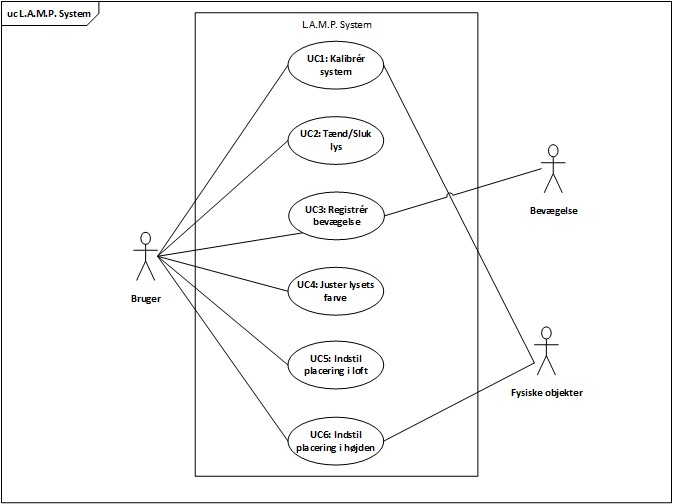
\includegraphics[width=\textwidth]{0_Filer/Figuer/ucLAMP2.jpg}
    \caption{Usecase diagram}
    \label{fig:usecasediagram}
\end{figure}

% UC1: Kalibrer system
\subsection{UC1: Kalibrer system}

\begin{center} \centering
	\begin{longtable}{|p{6cm}|p{8cm}|}
	\hline
		\multicolumn{2}{|l|}{\textbf{UC1: Kalibrer system}} \\\hline
		\endfirsthead
		
		\multicolumn{2}{l}{...fortsat fra forrige side} \\ \hline 
		\multicolumn{2}{|l|}{\textbf{UC1: Kalibrer system}} \\\hline
		\endhead	
		
		\multicolumn{2}{r}{fortsættes på næste side...} \\
        \endfoot
        \endlastfoot

        \textbf{Mål}								
            & Systemet bliver kalibreret og klar til brug.
        \\ \hline
        \textbf{Initialisering}					
            & Brugeren trykker på ”Kalibrer” på touchskærmen.
        \\ \hline
        \textbf{Aktører og Stakeholders}			
            & Bruger.
        \\ \hline
        \textbf{Referencer}						
            & Ingen.
        \\ \hline
        \textbf{Antal af samtidige hændelser}	
            & Ingen.
        \\ \hline
        \textbf{Forudsætning}					
            & Systemet er tændt og funktionsdygtigt.
        \\ \hline
        \textbf{Efterfølgende tilstand}			
            & Systemet er kalibreret og klar til brug.
        \\ \hline
        \textbf{Hovedforløb}						
            & 
            \begin{enumerate}
                \item Bruger trykker ”Kalibrer” på touchskærmen
                \item Z-Motor kører i top.
                \item Z-Motor registrerer når den rammer switchen i top, og sætter Z-værdien til nul på Z-PSoC'en
                \item X-motorerne kører i bund i den ene ende af skinnerne i loftet, og derefter til modsatte ende.
                \item Antal steps det tager X-motorerne at køre fra en ende til den anden gemmes på X-PSoC'en.
                \item Y-motoren kører i bund i den ene ende af skinnen, hvorefter den kører til den modsatte ende.
                \item Antal steps det tager Y-motorerne at køre fra en ende til den anden gemmes på Y-PSoC'en.
                \item Systemet er nu kalibreret og viser beskeden “Kalibrering udført” på touchskærmen.
            \end{enumerate}
        \\ \hline
        \textbf{Undtagelser}						
            & [Generel undtagelse 1: Kalibrering fejler]
            \begin{enumerate}
			    \item System stopper motorer
			    \item System viser beskeden “Kalibrering fejlet, tilkald tekniker” på touchskærmen.
		    \end{enumerate}
        \\ \hline
	\end{longtable}
	\label{UC1} 
\end{center}

% UC2: Tænd/Sluk lys
\subsection{UC2: Tænd/Sluk lys}

\begin{center} \centering
	\begin{longtable}{|p{6cm}|p{8cm}|}
	\hline
		\multicolumn{2}{|l|}{\textbf{UC2: Tænd/Sluk lys}} \\\hline
		\endfirsthead
		
		\multicolumn{2}{l}{...fortsat fra forrige side} \\ \hline 
		\multicolumn{2}{|l|}{\textbf{UC2: Tænd/Sluk lys}} \\\hline
		\endhead		

        \multicolumn{2}{r}{fortsættes på næste side...} \\
        \endfoot
        \endlastfoot
        
        \textbf{Mål}								
            & Brugeren får tændt eller slukket lampen.
        \\ \hline
        \textbf{Initialisering}					
            & Brugeren trykker på ”On”- eller ”Off”-knap på touchskærmen.
        \\ \hline
        \textbf{Aktører og Stakeholders}			
            & Bruger.
        \\ \hline
        \textbf{Referencer}						
            & Ingen.
        \\ \hline
        \textbf{Antal af samtidige hændelser}	
            & Ingen.
        \\ \hline
        \textbf{Forudsætning}					
            & Systemet er tændt og funktionsdygtigt. Touchskærmen viser 'Light'-fanen
        \\ \hline
        \textbf{Efterfølgende tilstand}			
            & Lampen har skiftet tilstand mellem slukket og tændt.
        \\ \hline
        \textbf{Hovedforløb}						
            & 
            \begin{enumerate}
                \item Brugeren indstiller en valgt farve via de tre RGB-sliders under 'Light'-fanen.
                \item Brugeren trykker Go-knappen.
                \item Brugeren trykker på ”On”- eller ”Off”-knap for lys.
                \item Lampen skifter tilstand.
            \end{enumerate}
        \\ \hline
        \textbf{Undtagelser}						
            & Ingen.
        \\ \hline
	\end{longtable}
	\label{UC2} 
\end{center}

% UC3: Registrér bevægelse
\subsection{UC3: Registrér bevægelse}

\begin{center} \centering
	\begin{longtable}{|p{6cm}|p{8cm}|}
	\hline
		\multicolumn{2}{|l|}{\textbf{UC3: Registrér bevægelse}} \\\hline
		\endfirsthead
		
		\multicolumn{2}{l}{...fortsat fra forrige side} \\ \hline 
		\multicolumn{2}{|l|}{\textbf{UC3: Registrér bevægelse}} \\\hline
		\endhead		

        \multicolumn{2}{r}{fortsættes på næste side...} \\
        \endfoot
        \endlastfoot
        
        \textbf{Mål}								
            & Systemet registrerer bevægelse og tænder Lampen.
        \\ \hline
        \textbf{Initialisering}					
            & Bevægelsessensor registrerer bevægelse.
        \\ \hline
        \textbf{Aktører og Stakeholders}			
            & Bevægelsessensor.
        \\ \hline
        \textbf{Referencer}						
            & Ingen.
        \\ \hline
        \textbf{Antal af samtidige hændelser}	
            & Ingen.
        \\ \hline
        \textbf{Forudsætning}					
            & Systemet er tændt og funktionsdygtigt. Touchskærmen viser 'Sensor'-fanen. Lampen er slukket og Movement detection slideren er sat til Off.
        \\ \hline
        \textbf{Efterfølgende tilstand}			
            & Lampen er tændt.
        \\ \hline
        \textbf{Hovedforløb}						
            &
            \begin{enumerate}
                \item Brugeren sætter Movement detection slideren på On.
                \item Bevægelsessensor registrerer bevægelse.
                \item Lampen tændes.
            \end{enumerate} 
        \\ \hline
        \textbf{Undtagelser}						
            & Ingen.
        \\ \hline
	\end{longtable}
	\label{UC3} 
\end{center}

% UC4: Juster lysets farve
\subsection{UC4: Juster lysets farve}

\begin{center} \centering
	\begin{longtable}{|p{6cm}|p{8cm}|}
	\hline
		\multicolumn{2}{|l|}{\textbf{UC4: Juster lysets farve}} \\\hline
		\endfirsthead
		
		\multicolumn{2}{l}{...fortsat fra forrige side} \\ \hline 
		\multicolumn{2}{|l|}{\textbf{UC4: Juster lysets farve}} \\\hline
		\endhead		

        \multicolumn{2}{r}{fortsættes på næste side...} \\
        \endfoot
        \endlastfoot
        
        \textbf{Mål}								
            & Brugeren får indstillet lysets farve til den valgte værdi.
        \\ \hline
        \textbf{Initialisering}					
            & Bruger trykker på touchskærmen.
        \\ \hline
        \textbf{Aktører og Stakeholders}			
            & Bruger.
        \\ \hline
        \textbf{Referencer}						
            & Ingen.
        \\ \hline
        \textbf{Antal af samtidige hændelser}	
            & Ingen.
        \\ \hline
        \textbf{Forudsætning}					
            & Systemet er tændt og funktionsdygtigt. Touchskærmen viser 'Light'-fanen.
        \\ \hline 
        \textbf{Efterfølgende tilstand}			
            & Brugeren har fået indstillet lysets farve til valgte tilstand.
        \\ \hline
        \textbf{Hovedforløb}						
            &
            \begin{enumerate}
                \item Bruger indstiller lysets farve på RGB-sliderne under 'Light'-fanen.
                \item Bruger trykker på Go-knappen.
                \item Lyset er nu justeret.
            \end{enumerate}
        \\ \hline
        \textbf{Undtagelser}						
            & Ingen.
        \\ \hline
	\end{longtable}
	\label{UC5} 
\end{center}

% UC5: Indstil placering af lampen
\subsection{UC5: Indstil placering i af lampen}

\begin{center} \centering
	\begin{longtable}{|p{6cm}|p{8cm}|}
	\hline
		\multicolumn{2}{|l|}{\textbf{UC5: Indstil placering af lampen}} \\\hline
		\endfirsthead
		
		\multicolumn{2}{l}{...fortsat fra forrige side} \\ \hline 
		\multicolumn{2}{|l|}{\textbf{UC5: Indstil placering af lampen}} \\\hline
		\endhead		

        \multicolumn{2}{r}{fortsættes på næste side...} \\
        \endfoot
        \endlastfoot
        
        \textbf{Mål}								
            & Brugeren har indstillet lampens placering i rummet.
        \\ \hline
        \textbf{Initialisering}					
            & Bruger trykker på touchskærmen.
        \\ \hline
        \textbf{Aktører og Stakeholders}			
            & Bruger.
        \\ \hline
        \textbf{Referencer}						
            & Ingen.
        \\ \hline
        \textbf{Antal af samtidige hændelser}	
            & Ingen.
        \\ \hline
        \textbf{Forudsætning}					
            & Systemet er tændt, kalibreret og funktionsdygtigt. Touchskærmen viser 'Position'-fanen.
        \\ \hline
        \textbf{Efterfølgende tilstand}			
            & Lampen hænger i en valgt position.
        \\ \hline
        \textbf{Hovedforløb}						
            &
            \begin{enumerate}
                \item Bruger sætter X, Y og Z sliderne til en valgt position under 'Position'-fanen.
                \item Bruger trykker på Go-knappen.
                \item Lampen flytter sig til den valgte position.
                [Undtagelse 1: Afstandssensor registrerer objekt]
            \end{enumerate}
        \\ \hline
        \textbf{Undtagelser}						
            & [Undtagelse 1: Afstandssensor registrerer objekt]
            \begin{enumerate}
			    \item System stopper Z-motoren.
			    \item Lampen hejses 1 cm op fra dens position.
		    \end{enumerate}
        \\ \hline
	\end{longtable}
	\label{UC6} 
\end{center}

% UC6: Indstil placering i loft
%\subsection{UC6: Indstil placering i højden}

\begin{center} \centering
	\begin{longtable}{|p{6cm}|p{8cm}|}
	\hline
		\multicolumn{2}{|l|}{\textbf{UC6: Indstil placering i højden}} \\\hline
		\endfirsthead
		
		\multicolumn{2}{l}{...fortsat fra forrige side} \\ \hline 
		\multicolumn{2}{|l|}{\textbf{UC6: Indstil placering i højden}} \\\hline
		\endhead		

        \multicolumn{2}{r}{fortsættes på næste side...} \\
        \endfoot
        \endlastfoot
        
        \textbf{Mål}								
            & Brugeren får hævet eller sænket lampen til den valgte højde.
        \\ \hline
        \textbf{Initialisering}					
            & Bruger trykker på touchskærmen.
        \\ \hline
        \textbf{Aktører og Stakeholders}			
            & Bruger.
        \\ \hline
        \textbf{Referencer}						
            & Ingen.
        \\ \hline
        \textbf{Antal af samtidige hændelser}	
            & Ingen.
        \\ \hline
        \textbf{Forudsætning}					
            & At systemet er tændt, kalibreret og funktionsdygtigt.
        \\ \hline		
        \textbf{Efterfølgende tilstand}	
            & Lampens højde er indstillet til det valgte niveau.
        \\ \hline
        \textbf{Hovedforløb}						
            &
            \begin{enumerate}
                \item Bruger ændre Z-slider positionen, i position tappen.
                \item Brugeren trykker på GO-kanppen, på position tappen. 
                    \newline [Undtagelse 1: Sensor registrerer forhindring]
                \item Lampe er nu indstillet til den valgte højde.
            \end{enumerate}
        \\ \hline
        \textbf{Undtagelser}						
            & [Undtagelse 1: Sensor registrerer forhindring]
            \begin{enumerate}
                \item Systemet stopper nedsænkningen af lampen og kan kun køre opad igen.
            \end{enumerate}
        \\ \hline
	\end{longtable}
	\label{UC7} 
\end{center}

% UC7: Indstil placering i højden
%\subsection{UC7: Tilføj plan}

\begin{center} \centering
	\begin{longtable}{|p{6cm}|p{8cm}|}
	\hline
		\multicolumn{2}{|l|}{\textbf{UC7: Tilføj plan}} \\\hline
		\endfirsthead
		
		\multicolumn{2}{l}{...fortsat fra forrige side} \\ \hline 
		\multicolumn{2}{|l|}{\textbf{UC7: Tilføj plan}} \\\hline
		\endhead		

        \multicolumn{2}{r}{fortsættes på næste side...} \\
        \endfoot
        \endlastfoot
        
        \textbf{Mål}								
            & En ny plan med position og lysindstillinger bliver oprettet på touchskærmen.
        \\ \hline
        \textbf{Initialisering}					
            & Bruger trykker på en plan under planner fanen på touchskærmen.
        \\ \hline
        \textbf{Aktører og Stakeholders}			
            & Bruger.
        \\ \hline
        \textbf{Referencer}						
            & Ingen.
        \\ \hline
        \textbf{Antal af samtidige hændelser}	
            & Ingen.
        \\ \hline
        \textbf{Forudsætning}					
            & At systemet er tændt og funktionsdygtigt.
        \\ \hline
        \textbf{Efterfølgende tilstand}			
            & En ny plan med systemets nuværende indstillinger er gemt på touchskærmen med et udvalgt navn.
        \\ \hline
        \textbf{Hovedforløb}						
            &
            \begin{enumerate}
                \item Bruger klikker Planner-fanen på touchskærmen.
                \item Bruger klikker ”Save location” på touchskærmen.
                \item Devkit8000 giver brugeren et nyt vindue hvor et udvalgt navn til planen kan indtastes
                \item Bruger indtaster et udvalgt navn i indtast- ningsfeltet ”Plan name:”.
                \item Bruger trykker på ”Save” i vinduet på touchskærmen.     \newline [Undtagelse 1: Bruger trykker ”Cancel”]
                \item Ny plan med udvalgte navn og nuværende indstillinger er oprettet og kan ses under Planner-fanen.
            \end{enumerate}
        \\ \hline
        \textbf{Undtagelser}						
            & [Undtagelse 1: Bruger trykker “Cancel”]
             \begin{enumerate}
                \item Bruger klikker på “Cancel”-knappen.
                \item Vinduet til oprettelse af plan på touchskærmen lukkes ned og ingen plan er gemt.
             \end{enumerate}
        \\ \hline
	\end{longtable}
	\label{UC8} 
\end{center}

% UC8: Tilføj plan
%\subsection{UC8: Vælg plan}

\begin{center} \centering
	\begin{longtable}{|p{6cm}|p{8cm}|}
	\hline
		\multicolumn{2}{|l|}{\textbf{UC8: Vælg plan}} \\\hline
		\endfirsthead
		
		\multicolumn{2}{l}{...fortsat fra forrige side} \\ \hline 
		\multicolumn{2}{|l|}{\textbf{UC8: Vælg plan}} \\\hline
		\endhead		

        \multicolumn{2}{r}{fortsættes på næste side...} \\
        \endfoot
        \endlastfoot
        
        \textbf{Mål}								
            & Systemet skifter position og lysindstillinger fra de nuværende til de udvalgte.
        \\ \hline
        \textbf{Initialisering}					
            & Bruger trykker på en plan under planner fanen på touchskærmen.
        \\ \hline
        \textbf{Aktører og Stakeholders}			
            & Bruger.
        \\ \hline
        \textbf{Referencer}						
            & Ingen.
        \\ \hline
        \textbf{Antal af samtidige hændelser}	
            & Ingen.
        \\ \hline
        \textbf{Forudsætning}					
            & At systemet er tændt, funktionsdygtigt, har en plan oprettet og har andre indstillinger end de udvalgte fra planen.
        \\ \hline
        \textbf{Efterfølgende tilstand}			
            & Systemet er nu indstillet til valgte tilstand.
        \\ \hline
        \textbf{Hovedforløb}						
            &
            \begin{enumerate}
                \item Bruger klikker Planner-fanen på touchskærmen.
                \item Bruger klikker en gemt plan på touchskærmen.
                \item Systemet er nu indstillet til indstillinger identiske til den udvalgte plan.
            \end{enumerate}
        \\ \hline
        \textbf{Undtagelser}						
            & Ingen.
        \\ \hline
	\end{longtable}
	\label{UC9} 
\end{center}

% UC9: Vælg plan
%\subsection{UC9: Vælg plan}

\begin{center} \centering
	\begin{longtable}{|p{6cm}|p{8cm}|}
	\hline
		\multicolumn{2}{|l|}{\textbf{UC9: Vælg plan}} \\\hline
		\endfirsthead
		
		\multicolumn{2}{l}{...fortsat fra forrige side} \\ \hline 
		\multicolumn{2}{|l|}{\textbf{UC9: Vælg plan}} \\\hline
		\endhead		

        \multicolumn{2}{r}{fortsættes på næste side...} \\
        \endfoot
        \endlastfoot
        
        \textbf{Mål}								
            & Systemet skifter position og lysindstillinger fra de nuværende til de udvalgte.
        \\ \hline
        \textbf{Initialisering}					
            & Bruger trykker på en plan under planner fanen på touchskærmen.
        \\ \hline
        \textbf{Aktører og Stakeholders}			
            & Bruger.
        \\ \hline
        \textbf{Referencer}						
            & Ingen.
        \\ \hline
        \textbf{Antal af samtidige hændelser}	
            & Ingen.
        \\ \hline
        \textbf{Forudsætning}					
            & At systemet er tændt, funktionsdygtigt, har en plan oprettet og har andre indstillinger end de udvalgte fra planen.
        \\ \hline
        \textbf{Efterfølgende tilstand}			
            & Systemet er nu indstillet til valgte tilstand.
        \\ \hline
        \textbf{Hovedforløb}						
            &
            \begin{enumerate}
                \item Bruger klikker Planner-fanen på touchskærmen.
                \item Bruger klikker en gemt plan på touchskærmen.
                \item Systemet er nu indstillet til indstillinger identiske til den udvalgte plan.
            \end{enumerate}
        \\ \hline
        \textbf{Undtagelser}						
            & Ingen.
        \\ \hline
	\end{longtable}
	\label{UC9} 
\end{center}